\section{Introduction}

\subsection{Dimensionality Reduction and Singular Value Decomposition}

In many applications data can be represented as a matrix that defines a mapping
between two feature spaces. As an example a dataset of ratings of users for
movies may be considered. As depicted in Figure~\ref{fig:exmpl_matrix}, such a
dataset can be modeled as a matrix in which each row represents a user, each
column a movie, and each value a rating that a user has given a movie.

\begin{figure}[h]
\centering
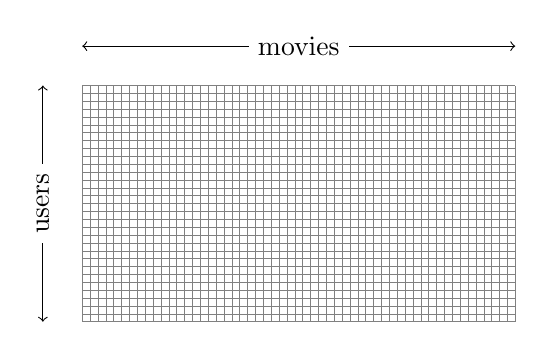
\begin{tikzpicture}
\draw[<->] (0,0.5) -- (0,3.5) node[pos=.5,sloped,fill=white] {users};
\draw[<->] (0.5,4) -- (6,4) node[pos=.5,sloped,fill=white] {movies};
%\draw      (0.5,0.5)  rectangle(6,3.5);
\draw[step=1mm,gray,very thin] (0.4999,0.4999) grid (6,3.5);
\end{tikzpicture}
\caption{Example of a matrix that represents a dataset of ratings from users
for movies}
\label{fig:exmpl_matrix}
\end{figure}

The general goal of such a matrix or vector representation of data is to
exploit well known mathematical functions and properties to process the data,
which is done by many machine learning and data mining algorithms. However, if
at least one feature space is very large, which means in the example that the
number of movies or users is very high, the practical application of this
approach is hindered. The most obvious reason for this roots in the size of the
data, that can get too large as to fit into main memory or as to be processed
efficiently. Beyond that a large number of (possibly dependent) dimensions can
render mathematical functions useless---especially vector distances, on which
important algorithms in machine learning and data mining rely. The latter class
of phenomena is grouped under the term \textsl{curse of dimensionality}.

One approach to tackle the aforementioned problems is called
\textsl{dimensionality reduction} and aims to compress the data's feature
spaces by reducing the number of their dimensions. For instance this would mean
in our example to compress the number of movies to a more abstract concept like
genres as depicted in Figure \ref{fig:exmpl_dr} (in reality, concepts are more
fuzzy than genres).

\begin{figure}[h]
\centering
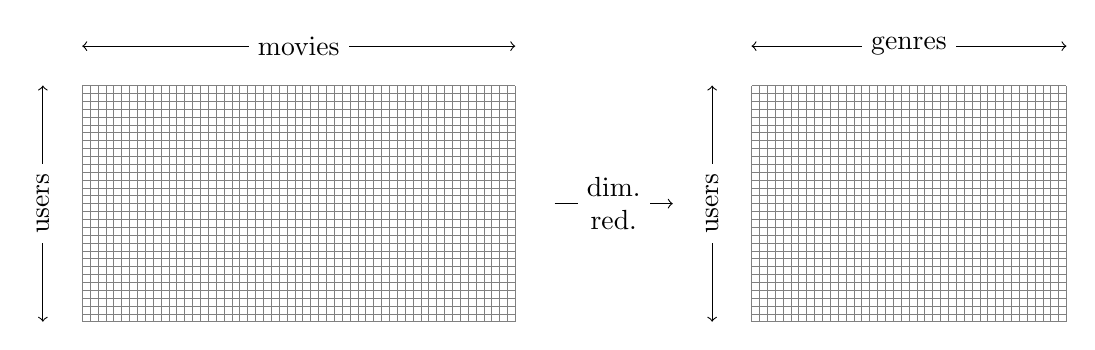
\begin{tikzpicture}
\draw[<->] (0,0.5) -- (0,3.5) node[pos=.5,sloped,fill=white] {users};
\draw[<->] (0.5,4) -- (6,4) node[pos=.5,sloped,fill=white] {movies};
\draw[step=1mm,gray,very thin] (0.4999,0.4999) grid (6,3.5);
\draw[->] (6.5,2) -- (8,2) node[pos=.5,sloped,fill=white, align=center] {dim.
\\ red.};
\draw[<->] (8.5,0.5) -- (8.5,3.5) node[pos=.5,sloped,fill=white] {users};
\draw[<->] (9,4) -- (13,4) node[pos=.5,sloped,fill=white] {genres};
\draw[step=1mm,gray,very thin] (8.9999,0.4999) grid (13,3.5);
\end{tikzpicture}
\caption{Example of dimensionality reduction used to compress the column
feature space from movies to genres}
\label{fig:exmpl_dr}
\end{figure}

This leads to an approximated view of the data, in which a set of movies are
grouped to one or more genres, that are liked or disliked by a set of users.
The approximated data can then be processed more efficiently and sometimes even
more precisely or in a more meaningful way. In \textsl{Latent Semantic
Indexing} for example, a set of documents is indexed by a set of abstract
concepts like topics that are more meaningful to a querying user than a set of
words. The astounding beauty of dimensionality reduction lies in the way it can
be achieved mathematically in an entirely domain agnostic way: With
dimensionality reduction hidden concepts like genres or topics can be
discovered in data that were previously unknown to an investigator. The
abstract concepts like genres or topics are not required to be known in advance
nor is the mapping of concrete feature space dimensions to concepts.

One way of achieving dimensionality reduction is to exploit the
\textsl{Singular Value Decomposition (SVD)} of a matrix. The SVD of a matrix
represents that matrix as a product of three special matrices:

\begin{equation}
	M = U \times \Sigma \times V^T
\end{equation}

$U$ is the basis of the row-feature space and $V$ is the basis of the
column-feature space. So $U$ consists of orthonormal eigenvectors of $M\times
M^T$ and $V$ consists of orthonormal eigenvectors of $M^T\times M$. A
mathematical intuition for this results from building the product of $M$ with
it's transpose and vice versa analog:

\begin{align*}
M \times M^T 	& = (U \times \Sigma \times V^T) \times (V \times \Sigma^T \times
U^T) \\
					& = (U \times \Sigma) \times (\Sigma^T \times U^T) \\
					& = U \times \Sigma^2 \times U^T
\end{align*}

So $U$ and $V$ are the eigendecompositions of $M\times M^T$ and $M^T\times M$
respectively. $\Sigma$ is a diagonal matrix that holds the corresponding
square-rooted eigenvalues in descending order. Figure \ref{fig:svd} gives a
more detailed view on the SVD of a matrix $M$.

\begin{figure}[h]
	\centering
	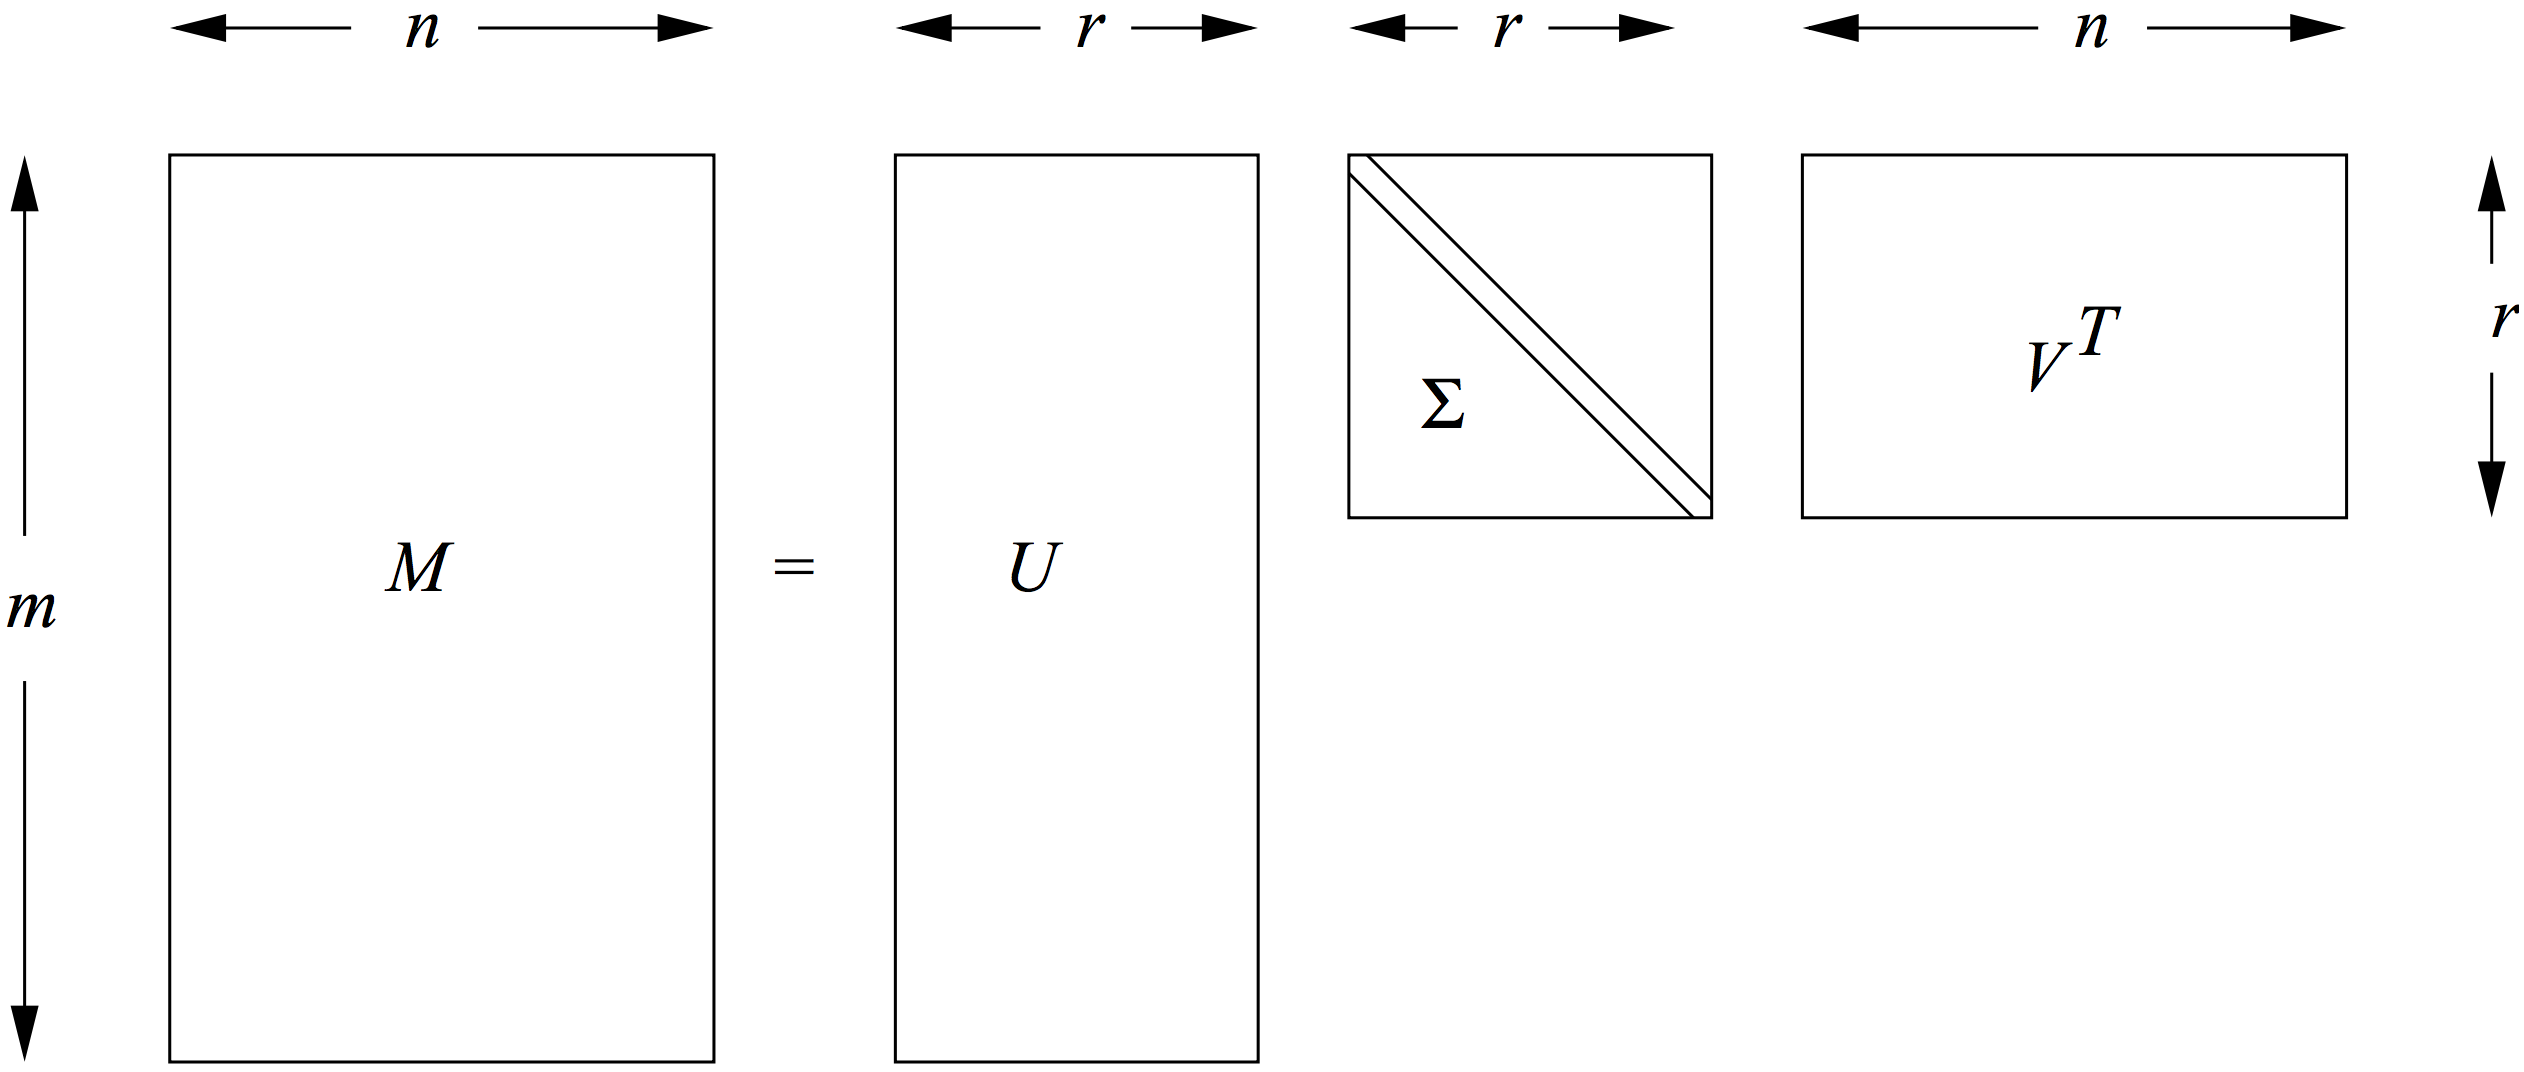
\includegraphics[width=0.8\textwidth]{images/svd_mmds.png}
\caption{Depiction of the SVD of a matrix $M$. Note that it is not necessarily
$r_n = r_m$}
	\label{fig:svd}
\end{figure}

The actual reduction of dimensions is then performed by dropping least
significant eigenvalues of $\Sigma$ along with corresponding eigenvectors in
$U$ and $V$ and keeping only the top $k$ one. The resulting matrix in then
called the $rank_k$ approximation of $M$. This works because the column vectors
of $U$ and $V$ and normalized and thus do not contribute value or length to a
recomposed element. That is entirely done by the eigenvalues of $\Sigma$. By
dropping the smallest values of those, a lowest possible approximation error is
ensured.

\subsection{The Lanczos Algorithm}
\label{ssec:lanczos_algorithm}

Computing the complete SVD of a large matrix is very expensive, especially if
considered that only the top $k$ eigenpairs are kept. Therefore the Lanczos
Algorithm is often used as an auxiliary tool, as it provides the possibility to
directly compute the top $k$ eigenpairs: The Lanczos algorithm takes as input a
matrix $A$ and computes as result a matrix $Q$ of Lanczos vectors and a
symmetric, tridiagonal auxiliary matrix $T$.

\begin{align*}
	Lanzcos(A) = (Q,T)
\end{align*}


%Another example for this approach is a dataset that contains for a corpus of
documents and a dictionary of words the number of how often a word appears in a
document. A matrix representation of this situation models i.e. documents as
rows, columns as words, and values as the sum of how often a word appears in a
document.

